\documentclass[11pt]{report}

\usepackage[utf8]{inputenc}
\usepackage[portuguese]{babel}
\usepackage[a4paper]{geometry}
\usepackage{todonotes}
\usepackage{url}
\usepackage{xcolor}
\usepackage{listings}
\usepackage{enumitem}
\usepackage{soul}
\usepackage{hyperref}
\usepackage{titling}
\usepackage{graphicx}

\graphicspath{ {images/} }

\begin{document}
\title{\textbf{BananaCore}\\{\LARGE Processador em VHDL}}
\author{
  Rogiel Sulzbach
  \and
  Jefferson Johner
  \and
  Matheus Oliveira
}
\date{\today}

\begin{titlepage} \center
	{
		UNIVERSIDADE FEDERAL DO RIO GRANDE DO SUL\\
		ESCOLA DE ENGENHARIA\\
		DEPARTAMENTO DE ENGENHARIA ELÉTRICA\\
		SISTEMAS DIGITAIS
	}
	
	\vfill
	
	{\Huge
		\thetitle
	}
	
	\vfill
	
	{\Large
		\theauthor
	}
	
	\vfill
	
	{\small
		\thedate
	}
\end{titlepage}

\tableofcontents

\chapter{Introdução}

O presente projeto versa sobre o processador BananaCore, desenvolvido como trabalho final da disciplina ENG04461 - Sistemas Digitais. Faz-se importante ressaltar que nosso processador foi desenvolvido com fins didáticos, não tentando priorizar desempenho ótimo.
Esse projeto tem um valor didático ainda maior para nós pois além de nos fazer trabalhar com a matéria de Sistemas Digitais e a linguagem de descrição VHDL, fez com que tenhamos ainda mais domínio sobre o conteúdo de Microcontroladores, que é uma área de grande importância para engenheiros eletricistas, mas que infelizmente o currículo de nosso curso não dá muita ênfase.

\chapter{Especificação}

A especificação inicial para o nosso projeto consiste em um processador de arquitetura do tipo Von Neumann\footnote{A arquitetura Von Neumann consiste em uma única memória compartilhada tanto para dados como para programas.} de 16 bits com instruções básicas do tipo:

\begin{itemize}
	\item Operações de memória: Carregar dado da memória, armazenar dado na memória
	\item Operações aritméticas: adição, subtração, multiplicação e divisão
	\item Operações de IO: Write port e Read port
	\item Operações bit-a-bit: AND, NAND, OR, NOR, XOR e NOT
\end{itemize}

Como o objetivo do trabalho é desenvolver apenas um processador -- não estamos interessados em como armazenar o programa no FPGA -- escolhemos por gravar o programa de forma fixa; isto é, o programa é armazenado direto na memória RAM como um valor inicial.

Sabendo da limitação desta implementação, o design deve permitir que seja fácil substituir esta implementação inicial por outra mais funcional e completa.

\chapter{Implementação}

\section{Controlador de Memória}
\label{sec:MemoryController}
O controlador de memória é a unidade que faz o intermédio ao acesso a memória do processador.Nele, a operação de escrita é validada e então enviada para um respectivo memory bank (ver seção \ref{sec:MemoryBank}).

O controlador é operado utilizando $5$ sinais:

\begin{description}
	\item[Endereço (entrada)] Recebe um valor de 16 bits que representa o endereço que memória que se deseja operar
	\item[Leitura de dados (saída)] Retorna o valor equivalente ao byte armazenado no endereço solicitado ou alta impedância (caso esteja executando uma operação se escrita)
	\item[Escrita de dados (entrada)] Recebe o byte que deseja-se escrever na memória
	\item[Operação (entrada)] Indica a operação desejada na memória RAM (escrita ou leitura)
	\item[Pronto (saída)] Uma flag que indica que a operação de leitura/escrita foi concluída com sucesso.
\end{description}

\subsection{Leitura na memória RAM}
\label{MemoryRead}
Para ler um byte da memória RAM, primeiramente seleciona-se o endereço desejado e atribui-se este valor ao barramento de endereços. Em seguida, o bit de operação é definido em modo leitura e aguarda-se um número arbitrário de clocks até que o sinal de pronto transicione para nível alto. No instante em que este sinal transiciona, o dado já está disponível na porta de leitura.

\subsection{Escrita na memória RAM}
Para escrever um byte na memória RAM, primeiramente seleciona-se o endereço desejado e atribui-se este valor ao barramento de endereços. Em seguida, no barramento de escrita de dados, o valor do byte é atribuido e o bit de operação é definido para uma operação do tipo \emph{WRITE}. Devido ao fato da memória RAM possuir um clock diferenciado do processador central, é necessário aguardar um intervalo arbitrário de ciclos de clock até que o sinal de pronto seja colocado em alto. Neste momento, já é possível iniciar a escrita do próximo byte da mesma maneira.

\subsection{Memory Bank}
\label{sec:MemoryBank}
O memory bank é uma entidade simples e serve como uma abstração para um módulo de memória RAM genérico. O otimizador do Quartus II, ao detectar a presença de um grande bloco de dados, automaticamente executa uma otimização e substitui este por um bloco de memória RAM.

\section{Controlador de Registrador}
Para evitar que fosse necessário injetar um grande número de sinais de acesso a dados, controle e status dos registradores, uma abstração semelhante ao acesso à memória foi criada para simplificar este desenvolvimento. Detalhes desta implementação serão omitidos, pois são muito semelhantes ao barramento de memória.

Há 16 registradores no processador, onde 14 são de propósito geral, um acumulador e um registrador de controle. Cada registrador é dado um nome, de 0 a 15, normalmente representado em forma binária de \texttt{0b0000} até \texttt{0b1111}.

\begin{description}[style=multiline,topsep=10pt,leftmargin=3.2cm]
	\item[0b0000--0b1101] Propósito geral
	\item[0b1110] Acumulador
	\item[0b1111] Controle
\end{description}

\section{Controlador de Instruções}
\label{sec:InstructionController}
O controlador de instruções é, sem dúvida, uma das partes com maior quantidade de código descrevendo hardware; isto se dá devido a uma dificuldade que encontramos ao implementar um barramento único de acesso à memória e aos registradores.

\subsection{Decodificador de instruções}
\label{sec:InstructionDecoder}
\todo{Escrever seção do decodificador de instruções}
O decodificador de instruções tem como função interpretar os dados lidos da memória e a partir deles, identificar qual instrução deve ser executada e os argumentos usados conforme a função a ser executada 

\subsection{Executor de instruções}
\label{sec:InstructionExecutor}
Cada instrução foi dividida em uma entidade chamada de \emph{executor}. Esta entidade é responsável por fazer o carregamento de dados, execução da instrução e armazenamento do resultado final. Devido a repetição de código nestes executores, utilizamos geradores para gerar grande parte do código de forma automática e simples (ver seção \ref{sec:CodeGeneration}).

\subsection{Acesso à memória}
\label{sec:MemoryAccess}

Inicialmente, pretendíamos implementar o acesso global a memória por via de um barramento delimitado por \emph{buffers tri-state}, contudo, esta implementação se mostrou muito complexa, pois ao incrementar as implementações de instruções do processador o barramento entrava em um estado inválido pois mais de dois sinais tentavam ser escritos no barramento em simultâneo. Acreditamos que estes problemas são devidos a falhas de design da arquitetura e que poderiam ser resolvidas escolhendo uma forma alternativa de implementação das instruções.

A solução desde problema, embora não seja ideal, foi simples: um grande MUX foi implementado de forma a fazer o "controle" de acesso ao barramento principal. Esta solução tem um grave problema: a necessidade de escrever código cresce muito em função da quantidade de instruções implementadas. Para um processador simples como o BananaCore isto pode não ser um problema muito relevante. Para implementações maiores, porém, isto pode ganhar uma faceta muito mais adversa. Como forma de solucionar, parcialmente, este empecilho, fizemos uso de artefatos de geração de código para gerar os muxes e demais condições do decodificador de instruções (ver seção \ref{sec:CodeGeneration}).

\section{Exemplo de funcionamento}

Os bits correspondentes ao programa são definidos na memória inicial no endereço $0$. Ao inicializar o processador, o \textbf{InstructionController} (seção \ref{sec:InstructionController}) é responsável por carregar os primeiros 4 bytes de dados da memória. Após o carregamento inicial, o controlador é responsável por decodificar o opcode\footnote{Opcode é o código de instrução, um código de 8 bits que dá "nome" a cada instrução do processador} e extrair cada argumento das instruções. Estes dados são salvos em um flip-flop para uso posterior.

No próximo estágio, o \textbf{InstructionExecutor} (seção \ref{sec:InstructionExecutor}) correspondente a instrução decodificada é ativado. Nele, os argumentos da instrução são passados e a execução da instrução começa. Cada instrução tem um comportamento diferente: instruções que dependem de dados registrados, primeiramente carregam seus registradores um a um. Instruções que armazenam a saída em algum registrador, fazem o armazenamento ao final da execução.

Ao final da execução da instrução, uma flag de pronto é levantada e o InstructionController continua com a execução da próxima instrução na memória (repetindo o processo especificado acima).

Para simplificar o entendimento do processador, utilizaremos um programa simples utilizado para os testes do processador. O programa faz o cálculo da operação de fatorial utilizando o seguinte programa:

\begin{lstlisting}[language=C++,caption={Exemplo de código utilizado pelo Assembler},stepnumber=1,numbers=left,showlines=true]
Assembler::Assembler(memoryStore)
	.readIO(REGISTER_0)
	.loadConstant(REGISTER_1, 0)
	.loadConstant(REGISTER_2, 1)
	.loadConstant(REGISTER_3, 1)

	.mark(loopAddress)

	.multiply(REGISTER_2, REGISTER_0)
	.loadRegister(REGISTER_2, REGISTER_ACCUMULATOR)

	.subtract(REGISTER_0, REGISTER_3)
	.loadRegister(REGISTER_0, REGISTER_ACCUMULATOR)

	.notEqual(REGISTER_0, REGISTER_1)
	.jumpIfCarry(loopAddress)

	.writeIO(REGISTER_2)

	.jump(0);
\end{lstlisting}

O programa completo montado, em notação binária, é expresso abaixo:

\begin{lstlisting}[breakatwhitespace=true,breakindent=0em,breaklines=true]
00000011 00000000 00000000 00100001 00000000 00000000 00000000 00100010 00000000 00000001 00000000 00100011 00000000 00000001 00010010 00100000 00000000 00000010 00001110 00010001 00000011 00000000 00000000 00001110 00110101 00000001 00100010 00000000 00001110 00000010 00100000 00100000 00000000 00000000 
\end{lstlisting}

No exemplo anterior, o \emph{assembler} feito em C++ foi usado para gerar um código binário para o processador. Este é um algoritmo muito simples para cálculo de fatorial.

Primeiramente, o processador carrega os primeiros 4 bytes da memória; estes bytes correspondem a:

\begin{lstlisting}
00000011 00000000 00000000 00100001
\end{lstlisting}

O decodificador extrai os seguintes parâmetros:
\begin{description}[style=multiline,topsep=10pt,leftmargin=5cm]
	\item[Opcode] \texttt{00000011} (READ\_IO)
	\item[Argumento 0] \texttt{\st{0000}\textbf{0000}}
\end{description}

Nesta instrução (de acordo com a documentação, ver seção \ref{ch:Instruction documentation}), os primeiros 4 bits do argumento 0 são ignorados. E os últimos 4 bits são correspondentes ao registrador de destino em que o conteúdo da porta externa deve ser copiado para. O decodificador também armazena o tamanho correspondente a instrução, neste caso, 2 bytes.

Após decodificado, o próximo estágio para para a ativação do executor da instrução, em que um bit interno é setado e a máquina de estados inteira da instrução inicia a execução.

Para esta instrução, o conteúdo da porta de entrada é primeiramente lido para um registrador interno e, no próximo ciclo e movido para o registrador 0000 de acordo com o argumento da instrução.

Ao final da execução, o registrador interno chamado \textbf{program counter} é incrementado o valor correspondente ao tamanho da instrução atual (isto é, pula para o endereço $2$) onde a próxima instrução a ser executada se encontra.

O próximo ciclo de execução executa o seguinte bloco de memória:
\begin{lstlisting}
00000000 00100001 00000000 00000000
\end{lstlisting}

O decodificador extrai os seguintes parâmetros:
\begin{description}[style=multiline,topsep=10pt,leftmargin=5cm]
	\item[Opcode] \texttt{00000000} (LOAD)
	\item[Argumento 0] \texttt{0010}
	\item[Argumento 1] \texttt{0001}
	\item[Argumento 2] \texttt{00000000 00000000}
\end{description}

No argumento 0, o tipo de LOAD é especificado. De acordo com a documentação (ver seção \ref{ch:Instruction documentation}), o tipo 0010 corresponde ao carregamento de uma constante. No argumento 1, o registrador de destino é especificado e no argumento 2 a constante de 16-bits a ser carregada é especificada.

Ao iniciar a execução da instrução, o executor imediatamente escreve no registrador \texttt{0001} o valor \texttt{00000000 00000000} e assim que completado, o controlador de instruções procede para a próxima instrução.

\section{Geração de código}
\label{sec:CodeGeneration}
Para gerar os códigos repetitivos e forma algorítmica, fizemos usos de duas ferramentas distintas: Cog\footnote{Cog é um aplicativo que executa programas Python contidos em comentários do código fonte e substitui sua saída ao final da execução. O programa está disponível publicamente \mbox{em \url{http://nedbatchelder.com/code/cog/}}} e um script personalizado de geração de executores de instruções.

Mais detalhes da geração de código podem ser extraídas do código fonte do projeto disponível no GitHub.

\section{Especificação final}
A especificação final para o nosso projeto consiste em um processador de arquitetura do tipo Von Neumann\footnote{A arquitetura Von Neumann consiste em uma única memória compartilhada tanto para dados como para programas.} de 16 bits com instruções básicas do tipo:

\begin{itemize}
	\item Operações de memória: Carregar dado da memória, armazenar dado na memória
	\item Operações aritméticas: adição, subtração, multiplicação e divisão
	\item Operações de IO: Write port e Read port
	\item Operações bit-a-bit: AND, NAND, OR, NOR, XOR e NOT
\end{itemize}

\chapter{Testes}
\section*{Considerações gerais}
Após a compilação do projeto realizamos testes com vetores de simulação para termos uma melhor visualização de como nosso processador executa suas operações, abaixo seguem alguns screenshots da simulação que julgamos importantes de serem compartilhados.

\section{Controlador de memória}

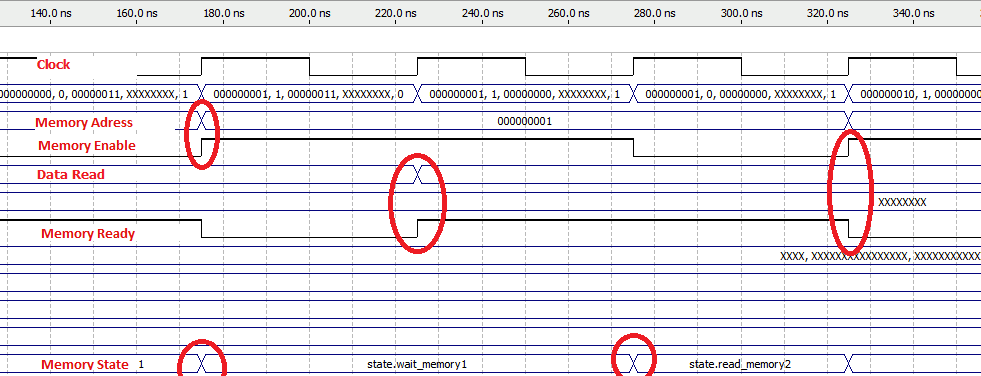
\includegraphics[width=\textwidth]{memory_controller}

Nessa imagem é fácil de entender como funciona o controlador de memória do processador (ver seção \ref{sec:MemoryAccess}). Na marca de 175ns um endereço de memória é fixado na entrada do controlador, após 1 ciclo de clock esse dado fica disponível na saída e a flag de memória pronta é levantada, no clock seguinte a memória e lida por fim a flag de memória pronta é baixada, um novo endereço é dado ao controlador de memória e o ciclo se repete.

\section{Instrução LOAD}

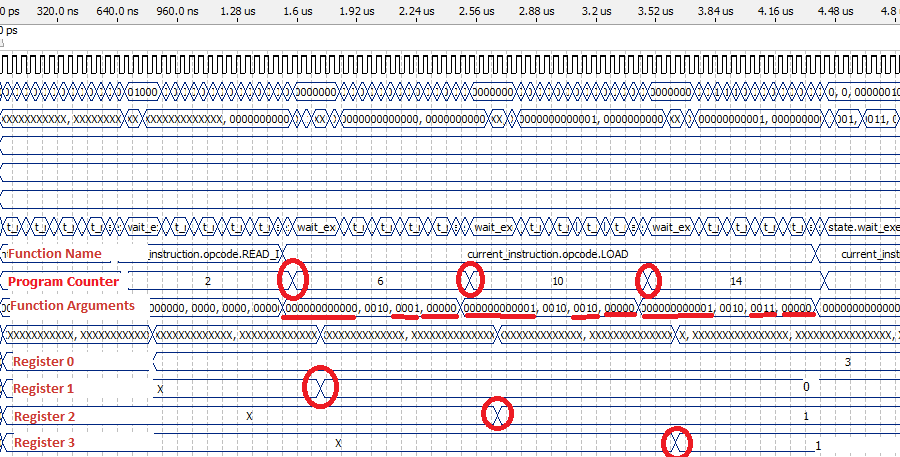
\includegraphics[width=\textwidth]{load}

Nessa imagem é fica claro o funcionamento da instrução LOAD para carregar dados nos registradores. Analisando o acréscimo do Program Counter percebe-se que essa instrução é executada 3 vezes entre as marcas de 1.28us e 4.48us

Nas 3 execuções dessa instrução o último argumento é 0000, o que indica que esta sendo feito o carregamento de um constante (indicada pelo primeiro argumento) em um registrador (indicado pelo terceiro argumento).

Em sua primeira execução o primeiro argumento é 0 e o terceiro é 1, o que indica que está sendo carregada a constante 0 no registrador 1, fato que pode ser comprovado ao analisar a alteração no dado do registrador 1.

Em sua segunda execução o primeiro argumento é 1 e o terceiro é 2, o que indica que está sendo carregada a constante 1 no registrador 2, fato que pode ser comprovado ao analisar a alteração no dado do registrador 2.

Em sua terceira execução o primeiro argumento é 1 e o terceiro é 3, o que indica que está sendo carregada a constante 1 no registrador 3, fato que pode ser comprovado ao analisar a alteração no dado do registrador 3.

Nesse intervalo estudado, a função LOAD carrega o registrador 1 com o valor 0 e os registradores 2 e 3 com o valor 1, como é dito no exemplo mostrado antes nesse relatório e pode ser percebido ao avaliar o valor dos registradores após o instante 4.16us.

\section{Instruções MULTIPLY}

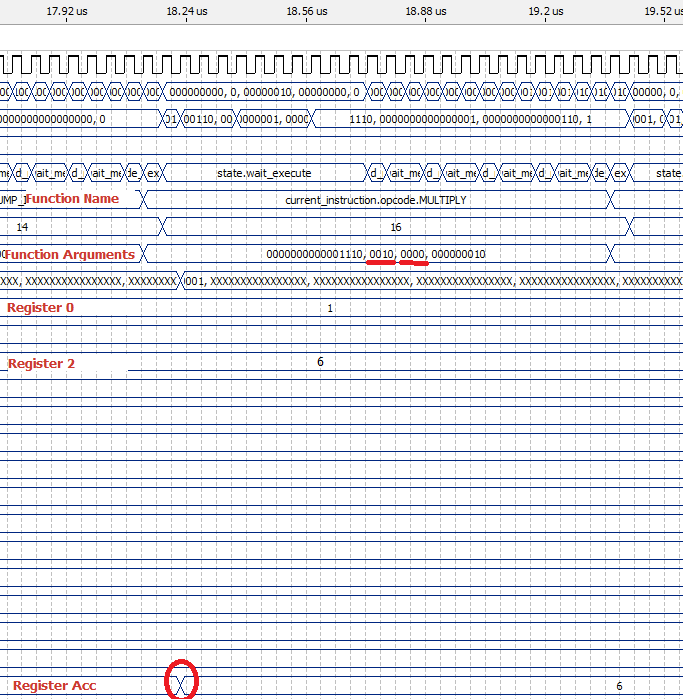
\includegraphics[width=\textwidth]{multiply}

Nessa imagem percebe-se o funcionamento da instrução MULTIPLY. Nessa instrução o valor armazenado no registrador referente ao segundo argumento é multiplicado com o valor do registrador do terceiro argumento e esse resultado é armazenado no registrador especial ACC.

Percebe-se que os argumentos dados são 2 e 0, assim essa instrução deve multiplicar os valores armazenados nos registradores 0 e 2 e salvar esse resultado no registrador ACC. O êxito da função é notado pela alteração do valor no registrador ACC para 6 no instante 18.24us

\section{Instrução NOT EQUAL}

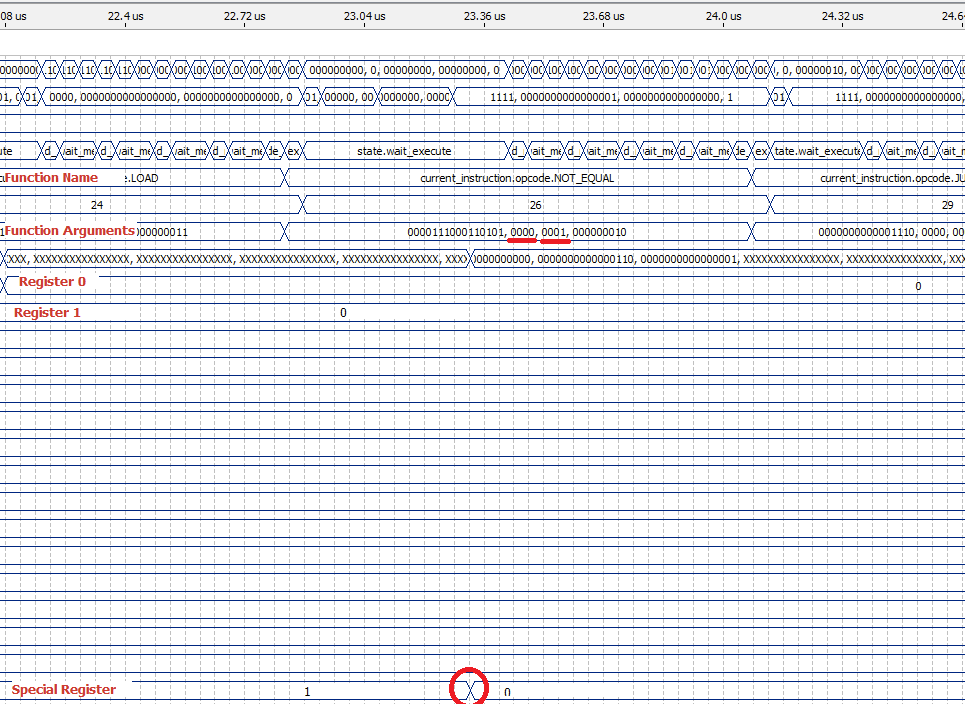
\includegraphics[width=\textwidth]{not_equal}

Nessa imagem o funcionamento da função NOT EQUAL fica bastante claro. Essa instrução compara os valores nos registradores indicados nos argumentos 2 e 3 e caso não sejam iguais seta o valor 1 no registrador especial.

Os argumentos dados para a função são 0 e 1, o que indica que os valores a serem comparados são os dos registradores 0 e 1. A função parece funcionar corretamente pois, após avaliar que os dois valores são iguais, seta o registrador especial para 0, no instante 23.36us.
\section*{Mais informações}
Caso deseje mais detalhes de nossos testes, o vetor de simulação .vwf, assim como todo o projeto, está disponível para consulta livre no repositório GitHub como especificado no capítulo seguinte.


\chapter{Código desenvolvido}
\label{ch:Instruction documentation}
Todo código VHDL, C++ e Python desenvolvido para este projeto está disponível livremente no GitHub.

\begin{description}
	\item[BananaCore] \url{https://github.com/Rogiel/BananaCore}
	\begin{description}
		\item[Documentação das instruções] \url{https://github.com/Rogiel/BananaCore/blob/master/Documentation/Instruction%20Set.md}
		\item[Vetor de simulação] \url{https://github.com/Rogiel/BananaCore/blob/master/Simulation}
	\end{description}
	
	\item[BananaVM] \url{https://github.com/Rogiel/BananaVM}
	\begin{description}
		\item[Assembler] \url{https://github.com/Rogiel/BananaVM/tree/master/Source/BananaVM/Assembler}
	\end{description}
\end{description}

\chapter{Melhoramentos futuros}
\section*{Tempos de espera redundantes}
Na implementação atual, o processador gasta muitos ciclos de clock esperando por sinais internos. Muitas destas esperas podem ser removidas ou simplificadas.

\section*{Aglutinação de leituras consecutivas}
Também, é possível aglutinar operações de forma simultânea. Por exemplo, é possível reduzir um ciclo de clock a cada leitura de 2 bytes consecutivos da memória ao iniciar a leitura do próximo imediatamente após a finalização da leitura anterior.

\section*{Acesso a memória em palavras maiores}
Para melhorar a performance é possível aumentar o tamanho da palavra retornada pelo controlador de memória. Atualmente o controlador retorna palavras com 8 bits. Este limite pode ser aumentado (ou configurável) de forma a permitir que seja possível ler mais bytes em apenas uma solicitação.

\section*{Ineficiência do divisor}
Após a análise de "slow-model" to TimeQuest, percebe-se claramente que o caminho crítico do processador está no divisor. Ele é responsável por um circuito síncrono, isto faz com que o clock do processador inteiro seja delimitado pelo clock deste caminho crítico. Uma possível solução seria implementar pipeline no cálculo da divisão para segmentar este caminho crítico em múltiplos caminhos menores.

\section*{Controlador de clock interno}
Se possível na placa de desenvolvimento, a criação de um controlador de clock interno permitiria que o clock fosse ajustado para velocidade mínima necessária no momento, bem como permitiria a redução (ou total desligamento) do clock do processador para economia de energia ou dissipação de calor.

\section*{Controlador de interrupções}
Uma futura melhoria interessante é a adição de interrupções por timers e externas.

\chapter{Conclusão}
Com este projeto pudemos adquirir conhecimentos sobre o projeto de um processador da arquitetura do tipo Von Neumann e experimentar formas de implementar o processador. Também adquirimos experiência na descrição de hardware digital em VHDL. Mais importante, pudemos constatar que a arquitetura escolhida, embora faça sentido ao iniciar o projeto, não foi a melhor escolha possível, visto que obtivemos baixa performance e alto \emph{overhead} ao executar as instruções.

Em especial, a escolha de implementar instruções com base em \emph{executors} não foi ideal, uma vez que abstrai muito a implementação física do hardware. Atribuímos este erro à falta de experiência -- nunca havíamos projetado um processador e a tarefa parece ser mais árdua do que aparenta.

Outro problema constatado após a implementado, foi a adoção de um barramento de registrador que provoca um atraso grande no processamento e impossibilita (ou ao menos dificulta bastante) a implementação de um pipeline de execução. Uma alternativa mais eficiente seria a conexão direta dos sinais de entrada, saída e controle de cada registrador diretamente aos operadores, sem a utilização de uma camada de indireção. Pelos resultados obtidos da simulação, tal implementação acarretaria num redução de até 60\% no número de ciclos por instrução para instruções com 2 argumentos registrados.

De forma geral, a especificação do conjunto de instruções esteja boa. O conjunto permite a execução de várias tarefas ainda que haja limitações no tipo de tarefas, como um pequeno e simples processador, acreditamos que a tarefa foi concluída de forma satisfatória.
\end{document}
